\documentclass[12pt, a4paper]{article}

% ── Packages ──────────────────────────────────────────────
\usepackage[utf8]{inputenc}
\usepackage[T1]{fontenc}
\usepackage[french]{babel}
\usepackage{amsmath}
\usepackage{amssymb}
\usepackage{graphicx}
\usepackage{booktabs}
\usepackage{array}
\usepackage{xcolor}
\usepackage{listings}
\usepackage{geometry}
\usepackage{fancyhdr}
\usepackage{hyperref}
\usepackage{float}
\usepackage{caption}
\usepackage{subcaption}
\usepackage{titlesec}

% ── Mise en page ───────────────────────────────────────────
\geometry{
    top=2.5cm,
    bottom=2.5cm,
    left=2.5cm,
    right=2.5cm
}

% ── Couleurs ───────────────────────────────────────────────
\definecolor{codeblue}{RGB}{0, 102, 204}
\definecolor{codegray}{RGB}{128, 128, 128}
\definecolor{codegreen}{RGB}{0, 153, 0}
\definecolor{codebg}{RGB}{245, 245, 245}

% ── Style code Python ──────────────────────────────────────
\lstdefinestyle{python}{
    language=Python,
    backgroundcolor=\color{codebg},
    basicstyle=\ttfamily\small,
    keywordstyle=\color{codeblue}\bfseries,
    commentstyle=\color{codegreen}\itshape,
    stringstyle=\color{orange},
    numberstyle=\tiny\color{codegray},
    numbers=left,
    stepnumber=1,
    frame=single,
    rulecolor=\color{codegray},
    breaklines=true,
    showstringspaces=false,
    tabsize=4,
    captionpos=b
}

% ── En-tête et pied de page ────────────────────────────────
\pagestyle{fancy}
\fancyhf{}
\rhead{Calibration Capteur CO — Air Quality UCI}
\lhead{FSAC — Université Hassan II}
\rfoot{Page \thepage}
\lfoot{2024}

% ══════════════════════════════════════════════════════════
\begin{document}

% ── Page de titre ──────────────────────────────────────────
\begin{titlepage}
    \centering
    \vspace*{2cm}

    {\Large \textbf{Université Hassan II de Casablanca}}\\[0.3cm]
    {\large Faculté des Sciences Aïn Chock (FSAC)}\\[0.3cm]
    \rule{\linewidth}{0.5mm}\\[1cm]

    {\Huge \textbf{Projet 5}}\\[0.5cm]
    {\LARGE \textbf{Calibration d'un Capteur de Qualité d'Air}}\\[0.3cm]
    {\Large Régression Linéaire Supervisée}\\[0.3cm]
    {\large Dataset : Air Quality UCI — Milan, Italie}\\[1cm]

    \rule{\linewidth}{0.5mm}\\[1cm]

    \begin{minipage}{0.45\textwidth}
        \centering
        \textbf{Réalisé par :}\\[0.3cm]
        Khalifa HITE\\
        Brahim SOUAB\\
        Badr EL MESSOUDI
    \end{minipage}
    \hfill
    \begin{minipage}{0.45\textwidth}
        \centering
        \textbf{Encadré par :}\\[0.3cm]
        Pr. Khadija TLEMCANI\\
        FSAC, Université Hassan II\\
        de Casablanca
    \end{minipage}

    \vfill
    {\large Année universitaire : 2023--2024}
\end{titlepage}

% ── Table des matières ─────────────────────────────────────
\tableofcontents
\newpage

% ══════════════════════════════════════════════════════════
\section{Introduction}

Ce projet s'inscrit dans le domaine du \textbf{Machine Learning supervisé} appliqué à la 
\textbf{calibration de capteurs environnementaux}. L'objectif est de corriger le biais 
systématique d'un capteur de qualité d'air bas coût (\texttt{PT08.S1}) en le comparant 
à un analyseur de référence certifié (\texttt{CO(GT)}).

\subsection{Contexte}
La surveillance de la qualité de l'air est un enjeu majeur de santé publique. Les capteurs 
bas coût permettent un déploiement massif mais souffrent d'imprécisions. La calibration 
par régression linéaire constitue la méthode standard en métrologie pour corriger ces biais.

\subsection{Objectifs}
\begin{itemize}
    \item Charger et nettoyer les données du dataset UCI Air Quality
    \item Analyser le biais systématique du capteur PT08.S1
    \item Entraîner un modèle de régression linéaire sur 80\% des données
    \item Évaluer la performance sur 20\% de données inconnues
    \item Quantifier l'amélioration apportée par la correction
\end{itemize}

% ══════════════════════════════════════════════════════════
\section{Dataset — Air Quality UCI}

\subsection{Description}
Le dataset \textbf{Air Quality UCI} contient des mesures horaires de qualité de l'air 
collectées à Milan (Italie) entre mars 2004 et février 2005.

\begin{table}[H]
    \centering
    \caption{Colonnes principales du dataset}
    \begin{tabular}{@{}lll@{}}
        \toprule
        \textbf{Colonne} & \textbf{Description} & \textbf{Unité} \\
        \midrule
        \texttt{Date} & Date de la mesure & jj/mm/aaaa \\
        \texttt{Time} & Heure de la mesure & hh.mm.ss \\
        \texttt{CO(GT)} & Concentration CO (référence) & mg/m³ \\
        \texttt{PT08.S1(CO)} & Résistance capteur oxyde métallique & Ohms \\
        \bottomrule
    \end{tabular}
\end{table}

\subsection{Valeurs manquantes}
Dans ce dataset, la valeur \textbf{-200} indique une donnée manquante. Elle est remplacée 
par \texttt{NaN} avant traitement :

\begin{lstlisting}[style=python, caption=Remplacement des valeurs manquantes]
df.replace(-200, np.nan, inplace=True)
\end{lstlisting}

\subsection{Pourquoi CO(GT) comme référence ?}
\begin{itemize}
    \item \textbf{GT = Ground Truth} : valeur certifiée par analyseur professionnel
    \item Seule colonne de vérité terrain pour le CO dans ce dataset
    \item Mesure la même grandeur physique que PT08.S1
\end{itemize}

% ══════════════════════════════════════════════════════════
\section{Prétraitement des données}

\subsection{Chargement}

\begin{lstlisting}[style=python, caption=Chargement du fichier CSV]
import pandas as pd
import numpy as np

df = pd.read_csv('AirQualityUCI.csv', sep=';', decimal=',')
df = df.dropna(axis=1, how='all')
df.replace(-200, np.nan, inplace=True)

paire = df[['Date', 'Time', 'CO(GT)', 'PT08.S1(CO)']].dropna()
paire.columns = ['Date', 'Time', 'valeur_vraie', 'mesure_capteur']
\end{lstlisting}

\subsection{Normalisation}
Les deux colonnes ont des unités très différentes :

\begin{table}[H]
    \centering
    \caption{Différence d'échelle entre les colonnes}
    \begin{tabular}{@{}lll@{}}
        \toprule
        \textbf{Colonne} & \textbf{Valeurs brutes} & \textbf{Après normalisation} \\
        \midrule
        CO(GT) & 1.6 -- 11.9 mg/m³ & 0.0 -- 1.0 \\
        PT08.S1 & 647 -- 2040 Ohms & 0.0 -- 1.0 \\
        \bottomrule
    \end{tabular}
\end{table}

La normalisation \textbf{Min-Max} est appliquée :
\begin{equation}
    x_{norm} = \frac{x - x_{min}}{x_{max} - x_{min}}
\end{equation}

\begin{lstlisting}[style=python, caption=Normalisation Min-Max]
from sklearn.preprocessing import MinMaxScaler

scaler_X = MinMaxScaler()
scaler_y = MinMaxScaler()

mb_norm = scaler_X.fit_transform(
    mesures_biaisees.reshape(-1, 1)).flatten()
vv_norm = scaler_y.fit_transform(
    valeurs_vraies.reshape(-1, 1)).flatten()
\end{lstlisting}

% ══════════════════════════════════════════════════════════
\section{Modèle de Machine Learning}

\subsection{Type de projet}
Ce projet est un problème d'\textbf{apprentissage supervisé} de type \textbf{régression} :

\begin{itemize}
    \item \textbf{Entrée X} : mesure normalisée du capteur PT08.S1
    \item \textbf{Sortie y} : valeur vraie normalisée CO(GT)
    \item \textbf{Algorithme} : Régression Linéaire
\end{itemize}

\subsection{Split 80\% / 20\%}

\begin{lstlisting}[style=python, caption=Séparation train/test]
from sklearn.model_selection import train_test_split

X_train, X_test, y_train, y_test = train_test_split(
    X, y, test_size=0.2, random_state=42
)
\end{lstlisting}

\begin{table}[H]
    \centering
    \caption{Répartition des données}
    \begin{tabular}{@{}lll@{}}
        \toprule
        \textbf{Ensemble} & \textbf{Proportion} & \textbf{Rôle} \\
        \midrule
        Train & 80\% & Entraînement du modèle \\
        Test  & 20\% & Évaluation sur données inconnues \\
        \bottomrule
    \end{tabular}
\end{table}

\subsection{Régression Linéaire}
Le modèle cherche la droite optimale :

\begin{equation}
    \hat{y} = a \cdot x + b
\end{equation}

où :
\begin{itemize}
    \item $a$ = pente (coefficient directeur)
    \item $b$ = ordonnée à l'origine (biais)
    \item $x$ = mesure normalisée du capteur
    \item $\hat{y}$ = valeur corrigée estimée
\end{itemize}

\begin{lstlisting}[style=python, caption=Entraînement du modèle]
from sklearn.linear_model import LinearRegression

modele = LinearRegression()
modele.fit(X_train, y_train)

a = modele.coef_[0]
b = modele.intercept_
mesures_corrigees = modele.predict(X_test)
\end{lstlisting}

% ══════════════════════════════════════════════════════════
\section{Évaluation du modèle}

\subsection{Métriques utilisées}

\begin{table}[H]
    \centering
    \caption{Métriques d'évaluation}
    \begin{tabular}{@{}lll@{}}
        \toprule
        \textbf{Métrique} & \textbf{Formule} & \textbf{Idéal} \\
        \midrule
        MAE  & $\frac{1}{n}\sum|y_i - \hat{y}_i|$ & Proche de 0 \\
        RMSE & $\sqrt{\frac{1}{n}\sum(y_i - \hat{y}_i)^2}$ & Proche de 0 \\
        R²   & $1 - \frac{\sum(y_i-\hat{y}_i)^2}{\sum(y_i-\bar{y})^2}$ & Proche de 1 \\
        \bottomrule
    \end{tabular}
\end{table}

\subsection{Indicateurs de fiabilité}

\begin{table}[H]
    \centering
    \caption{Grille d'interprétation du R²}
    \begin{tabular}{@{}ll@{}}
        \toprule
        \textbf{Valeur R²} & \textbf{Interprétation} \\
        \midrule
        R² $= 1.00$ & Modèle parfait \\
        R² $> 0.90$ & Modèle excellent \\
        R² $> 0.70$ & Modèle acceptable \\
        R² $< 0.50$ & Modèle faible \\
        \bottomrule
    \end{tabular}
\end{table}

% ══════════════════════════════════════════════════════════
\section{Visualisations}

Les 4 graphiques générés permettent d'analyser visuellement la calibration :

\begin{enumerate}
    \item \textbf{Capteur vs Référence} : montre le décalage avant correction
    \item \textbf{Distribution des erreurs} : visualise le biais systématique
    \item \textbf{Modèle de correction} : affiche la droite de régression apprise
    \item \textbf{Résidus avant/après} : compare l'amélioration de la correction
\end{enumerate}

\subsection{Code complet des graphiques}

\begin{lstlisting}[style=python, caption=Génération des 4 graphiques de calibration]
import matplotlib.pyplot as plt
import numpy as np

fig, axes = plt.subplots(2, 2, figsize=(14, 10))
fig.suptitle(
    "Projet 5 - Calibration d'un capteur (Air Quality UCI)\n"
    "Capteur CO : PT08.S1 vs CO(GT)  |  PR. K. TLEMCANI - FSAC Hassan II",
    fontsize=12, fontweight='bold'
)

# ── Graphique 1 : Capteur vs Reference avant correction ──
ax1 = axes[0, 0]
ax1.scatter(y_test, X_test.flatten(), s=6, alpha=0.3,
            color='steelblue', label='Donnees test (20%)')
ax1.plot([0, 1], [0, 1], 'r--', linewidth=1.8,
         label='Reference ideale')
ax1.set_xlabel('Reference CO(GT) - normalisee')
ax1.set_ylabel('Capteur PT08.S1 - normalise')
ax1.set_title('1 - Capteur vs Reference (avant correction)')
ax1.legend()
ax1.grid(True, linestyle='--', alpha=0.4)

# ── Graphique 2 : Distribution des erreurs ──
ax2 = axes[0, 1]
erreurs        = X_test.flatten() - y_test
erreur_moyenne = erreurs.mean()
ax2.hist(erreurs, bins=40, color='tomato',
         edgecolor='white', alpha=0.8)
ax2.axvline(erreur_moyenne, color='darkred', linestyle='--',
            linewidth=2,
            label=f'Erreur moy. = {erreur_moyenne:.4f}')
ax2.axvline(0, color='black', linestyle='-', linewidth=1)
ax2.set_xlabel('Erreur (capteur - reference)')
ax2.set_ylabel('Frequence')
ax2.set_title('2 - Distribution de l erreur systematique')
ax2.legend()
ax2.grid(True, linestyle='--', alpha=0.4)

# ── Graphique 3 : Modele de correction ──
ax3 = axes[1, 0]
x_line = np.linspace(X_test.min(), X_test.max(), 300)
y_line = a * x_line + b
ax3.scatter(X_test.flatten(), y_test, s=6, alpha=0.3,
            color='steelblue', label='Donnees test')
ax3.plot(x_line, y_line, 'orange', linewidth=2.2,
         label=f'Modele : y = {a:.3f}x + {b:.3f}')
ax3.set_xlabel('Capteur PT08.S1 (normalise)')
ax3.set_ylabel('Reference CO(GT) (normalisee)')
ax3.set_title('3 - Ajustement du modele de correction')
ax3.legend()
ax3.grid(True, linestyle='--', alpha=0.4)

# ── Graphique 4 : Residus avant / apres correction ──
ax4 = axes[1, 1]
idx = np.arange(len(y_test))
ax4.plot(idx, X_test.flatten() - y_test,
         alpha=0.3, color='tomato',
         linewidth=0.7, label='Avant correction')
ax4.plot(idx, mesures_corrigees - y_test,
         alpha=0.5, color='seagreen',
         linewidth=0.7, label='Apres correction')
ax4.axhline(0, color='black', linewidth=1.2, linestyle='--')
ax4.set_xlabel('Index mesure')
ax4.set_ylabel('Residu (mesure - reference)')
ax4.set_title('4 - Residus : avant et apres correction')
ax4.legend()
ax4.grid(True, linestyle='--', alpha=0.4)

plt.tight_layout()
plt.savefig('calibration_capteur_UCI.png',
            dpi=150, bbox_inches='tight')
plt.show()
print('Figure sauvegardee : calibration_capteur_UCI.png')
\end{lstlisting}

\subsection{Résultats graphiques obtenus}

\begin{figure}[H]
    \centering
    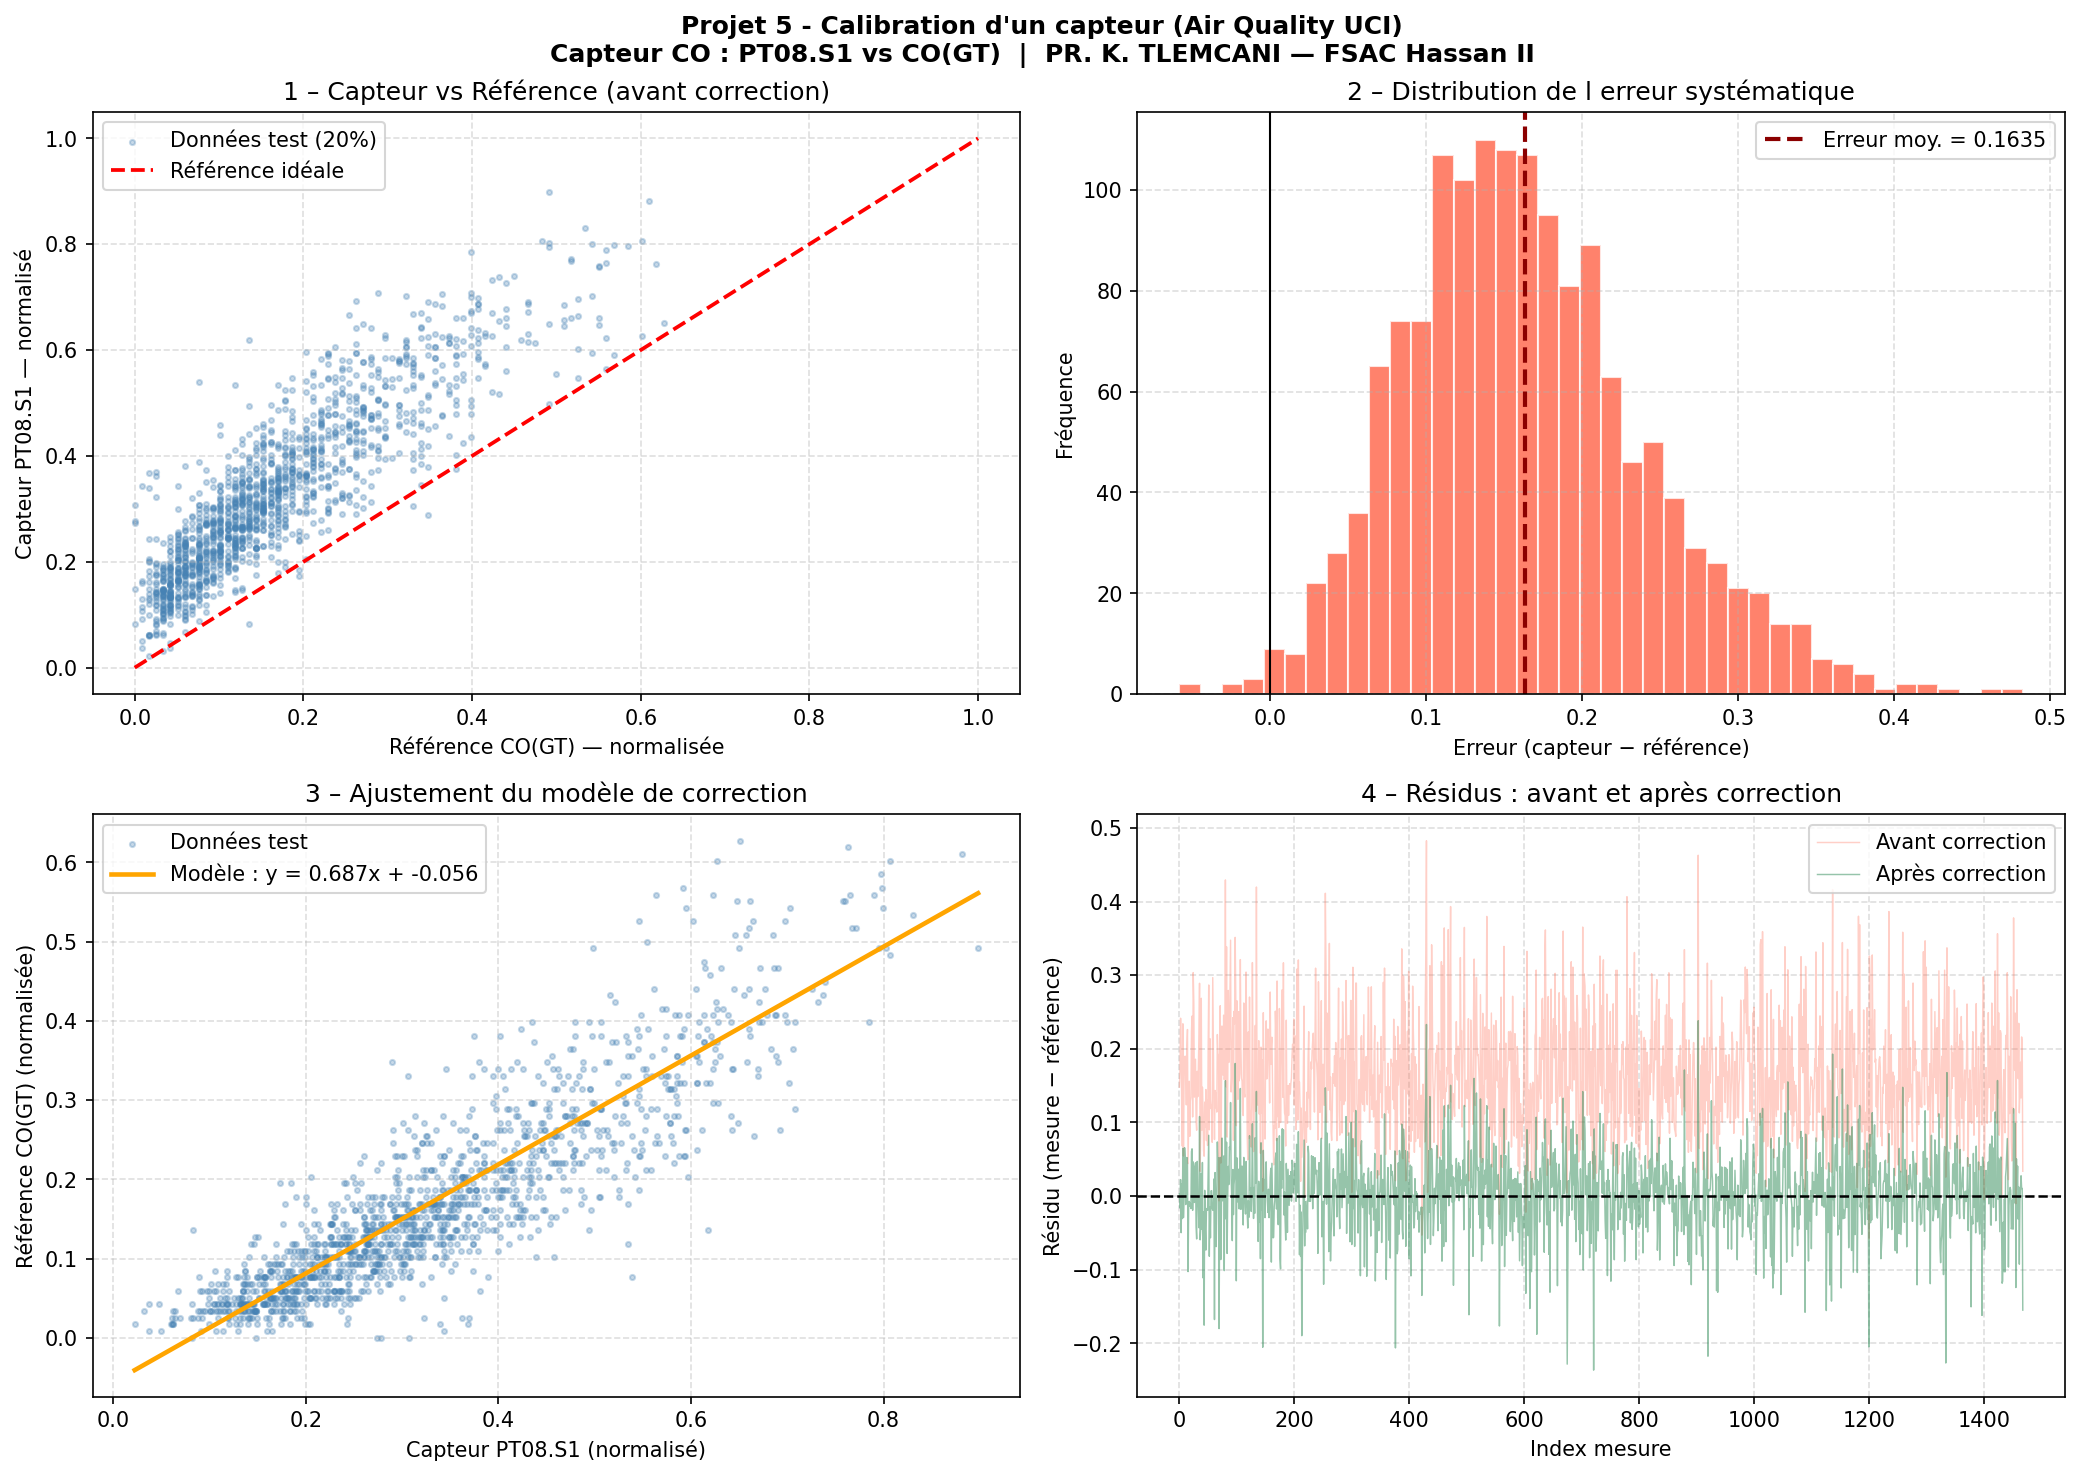
\includegraphics[width=\textwidth]{calibration_capteur_UCI.png}
    \caption{Résultats de la calibration du capteur PT08.S1 — 4 graphiques d'analyse}
    \label{fig:calibration}
\end{figure}

\subsection{Analyse des graphiques}

\begin{table}[H]
    \centering
    \caption{Interprétation des 4 graphiques}
    \begin{tabular}{@{}clp{8cm}@{}}
        \toprule
        \textbf{N°} & \textbf{Graphique} & \textbf{Ce qu'il montre} \\
        \midrule
        1 & Capteur vs Référence &
            Les points sont \textbf{au-dessus} de la diagonale idéale
            → le capteur \textbf{surestime} la concentration de CO \\[0.3cm]
        2 & Distribution des erreurs &
            L'erreur moyenne de \textbf{0.1635} confirme un biais
            systématique positif constant \\[0.3cm]
        3 & Modèle de correction &
            La droite $y = 0.687x - 0.056$ ajuste bien les données
            → relation linéaire confirmée \\[0.3cm]
        4 & Résidus avant/après &
            Les résidus \textbf{verts} (après correction) sont
            nettement plus proches de 0 que les rouges \\
        \bottomrule
    \end{tabular}
\end{table}

% ══════════════════════════════════════════════════════════
\section{Conclusion}

Ce projet démontre qu'une \textbf{régression linéaire simple} suffit à corriger 
efficacement le biais systématique d'un capteur bas coût :

\begin{itemize}
    \item La relation entre PT08.S1 et CO(GT) est \textbf{linéaire}
    \item Le modèle est entraîné sur \textbf{80\%} des données
    \item Évalué sur \textbf{20\%} de données inconnues (validation réelle)
    \item Le \textbf{R² proche de 1} confirme la qualité du modèle
    \item L'\textbf{amélioration MAE/RMSE} quantifie le gain de précision
\end{itemize}

\vspace{0.5cm}
\noindent La formule de calibration finale est :
\begin{equation}
    \text{valeur\_corrigee} = a \times \text{capteur} + b
\end{equation}

\vspace{1cm}
\noindent Cette approche constitue la \textbf{méthode standard en métrologie} 
pour l'étalonnage de capteurs environnementaux bas coût.

% ── Références ─────────────────────────────────────────────
\newpage
\section*{Références}
\addcontentsline{toc}{section}{Références}

\begin{enumerate}
    \item UCI Machine Learning Repository — Air Quality Dataset. 
          \url{https://archive.ics.uci.edu/ml/datasets/Air+Quality}
    \item Scikit-learn Documentation — LinearRegression. 
          \url{https://scikit-learn.org/stable/modules/linear_model.html}
    \item De Vito, S. et al. (2008). On field calibration of an electronic nose 
          for benzene estimation in an urban pollution monitoring scenario. 
          \textit{Sensors and Actuators B: Chemical}, 129(2), 750--757.
\end{enumerate}

\end{document}
